\documentclass[tikz,border=6pt]{standalone}
\usepackage{xcolor}
\begin{document}
% Canonical ch-diagram for 8_1^1,1
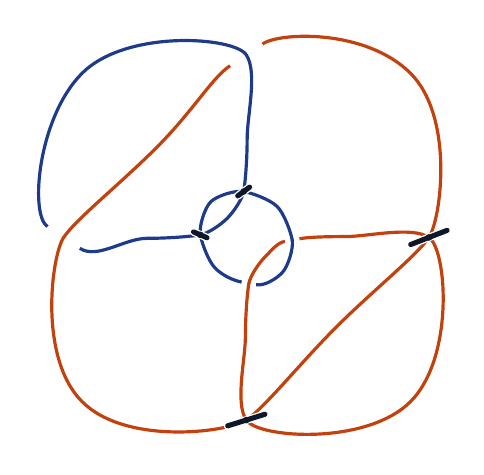
\begin{tikzpicture}[line join=round]
  \definecolor{skcomp0}{RGB}{30,58,138}
  \definecolor{skcomp1}{RGB}{194,65,12}
  \definecolor{skmark}{RGB}{15,23,42}
  \draw[skcomp0, line width=1.15pt, line cap=butt] (-2.4687,0.1378) .. controls (-2.7000,0.2929) and (-2.5878,1.5265) .. (-2.0291,2.0852);
  \draw[skcomp0, line width=1.15pt, line cap=butt] (-2.0576,-0.1378) .. controls (-1.8392,-0.2843) and (-1.4898,-0.0112) .. (-1.2051,-0.0112);
  \draw[skcomp1, line width=1.15pt, line cap=butt] (-0.1495,2.1814) .. controls (-0.3808,2.0263) and (-0.6216,1.6035) .. (-1.0845,1.1406);
  \draw[skcomp1, line width=1.15pt, line cap=butt] (0.2617,2.4571) .. controls (0.4929,2.6122) and (1.5825,2.6439) .. (2.1413,2.0852);
  \draw[skcomp1, line width=1.15pt, line cap=butt] (0.7314,-0.0165) .. controls (0.8348,0.0022) and (1.0325,0.0112) .. (1.3172,0.0112);
  \draw[skcomp0, line width=1.15pt, line cap=butt] (-0.0027,-0.5669) .. controls (-0.1060,-0.5482) and (-0.2471,-0.4819) .. (-0.3364,-0.3925);
  \draw[skcomp1, line width=1.15pt, line cap=butt] (0.5477,-0.0497) .. controls (0.4501,-0.0673) and (0.3782,-0.1626) .. (0.2984,-0.2424);
  \draw[skcomp0, line width=1.15pt, line cap=butt] (0.1810,-0.6001) .. controls (0.2844,-0.6187) and (0.4291,-0.5311) .. (0.5081,-0.4520);
  \draw[skcomp0, line width=1.15pt, line cap=round] (0.0561,2.3192) .. controls (-0.0990,2.5505) and (-1.4704,2.6439) .. (-2.0291,2.0852);
  \draw[skcomp1, line width=1.15pt, line cap=round] (-2.2632,0.0000) .. controls (-2.4182,-0.2313) and (-2.5878,-1.5265) .. (-2.0291,-2.0852);
  \draw[skcomp1, line width=1.15pt, line cap=round] (0.0561,-2.3192) .. controls (-0.1752,-2.4743) and (-1.4704,-2.6439) .. (-2.0291,-2.0852);
  \draw[skcomp0, line width=1.15pt, line cap=round] (-0.5274,0.0331) .. controls (-0.6307,0.0144) and (-0.9204,-0.0112) .. (-1.2051,-0.0112);
  \draw[skcomp1, line width=1.15pt, line cap=round] (-2.2632,0.0000) .. controls (-2.1081,0.2313) and (-1.5474,0.6776) .. (-1.0845,1.1406);
  \draw[skcomp0, line width=1.15pt, line cap=round] (0.0561,2.3192) .. controls (0.2025,2.1008) and (0.0673,1.5458) .. (0.0673,1.2611);
  \draw[skcomp0, line width=1.15pt, line cap=round] (0.0230,0.5835) .. controls (0.0417,0.6868) and (0.0673,0.9764) .. (0.0673,1.2611);
  \draw[skcomp1, line width=1.15pt, line cap=round] (2.3753,-0.0000) .. controls (2.5304,0.2313) and (2.7000,1.5265) .. (2.1413,2.0852);
  \draw[skcomp1, line width=1.15pt, line cap=round] (2.3753,-0.0000) .. controls (2.1569,0.1465) and (1.6019,0.0112) .. (1.3172,0.0112);
  \draw[skcomp1, line width=1.15pt, line cap=round] (2.3753,-0.0000) .. controls (2.2202,-0.2313) and (1.6596,-0.6776) .. (1.1966,-1.1406);
  \draw[skcomp1, line width=1.15pt, line cap=round] (0.0561,-2.3192) .. controls (0.2874,-2.1642) and (0.7337,-1.6035) .. (1.1966,-1.1406);
  \draw[skcomp1, line width=1.15pt, line cap=round] (2.3753,-0.0000) .. controls (2.6066,-0.1551) and (2.7000,-1.5265) .. (2.1413,-2.0852);
  \draw[skcomp1, line width=1.15pt, line cap=round] (0.0561,-2.3192) .. controls (0.2112,-2.5505) and (1.5825,-2.6439) .. (2.1413,-2.0852);
  \draw[skcomp1, line width=1.15pt, line cap=round] (0.0561,-2.3192) .. controls (-0.0904,-2.1008) and (0.0449,-1.5458) .. (0.0449,-1.2611);
  \draw[skcomp1, line width=1.15pt, line cap=round] (0.0892,-0.5835) .. controls (0.0705,-0.6868) and (0.0449,-0.9764) .. (0.0449,-1.2611);
  \draw[skcomp0, line width=1.15pt, line cap=round] (-0.5274,0.0331) .. controls (-0.5087,-0.0703) and (-0.4258,-0.3032) .. (-0.3364,-0.3925);
  \draw[skcomp0, line width=1.15pt, line cap=round] (-0.5274,0.0331) .. controls (-0.4298,0.0507) and (-0.2660,0.1626) .. (-0.1863,0.2424);
  \draw[skcomp0, line width=1.15pt, line cap=round] (0.0230,0.5835) .. controls (0.0054,0.4859) and (-0.1066,0.3221) .. (-0.1863,0.2424);
  \draw[skcomp0, line width=1.15pt, line cap=round] (-0.5274,0.0331) .. controls (-0.5461,0.1364) and (-0.4750,0.3730) .. (-0.3960,0.4520);
  \draw[skcomp0, line width=1.15pt, line cap=round] (0.0230,0.5835) .. controls (-0.0804,0.6021) and (-0.3169,0.5311) .. (-0.3960,0.4520);
  \draw[skcomp0, line width=1.15pt, line cap=round] (0.0230,0.5835) .. controls (0.1263,0.5648) and (0.3593,0.4819) .. (0.4486,0.3925);
  \draw[skcomp0, line width=1.15pt, line cap=round] (0.6396,-0.0331) .. controls (0.6209,0.0703) and (0.5379,0.3032) .. (0.4486,0.3925);
  \draw[skcomp1, line width=1.15pt, line cap=round] (0.0892,-0.5835) .. controls (0.1068,-0.4859) and (0.2187,-0.3221) .. (0.2984,-0.2424);
  \draw[skcomp0, line width=1.15pt, line cap=round] (0.6396,-0.0331) .. controls (0.6582,-0.1364) and (0.5871,-0.3730) .. (0.5081,-0.4520);
  \draw[white, line width=2.8pt, line cap=round] (2.6059,0.0899) -- (2.1447,-0.0899);
  \draw[skmark, line width=1.85pt, line cap=round] (2.6059,0.0899) -- (2.1447,-0.0899);
  \fill[skmark] (2.3753,-0.0000) circle (1.2pt);
  \draw[white, line width=2.8pt, line cap=round] (-0.1803,-2.3927) -- (0.2924,-2.2457);
  \draw[skmark, line width=1.85pt, line cap=round] (-0.1803,-2.3927) -- (0.2924,-2.2457);
  \fill[skmark] (0.0561,-2.3192) circle (1.2pt);
  \draw[white, line width=2.8pt, line cap=round] (-0.6131,0.0702) -- (-0.4417,-0.0040);
  \draw[skmark, line width=1.85pt, line cap=round] (-0.6131,0.0702) -- (-0.4417,-0.0040);
  \fill[skmark] (-0.5274,0.0331) circle (1.2pt);
  \draw[white, line width=2.8pt, line cap=round] (0.0983,0.6386) -- (-0.0523,0.5283);
  \draw[skmark, line width=1.85pt, line cap=round] (0.0983,0.6386) -- (-0.0523,0.5283);
  \fill[skmark] (0.0230,0.5835) circle (1.2pt);
\end{tikzpicture}
\end{document}
